\documentclass[12pt,twoside, a4paper, twocolumn]{article}
\usepackage[utf8]{inputenc}
\usepackage[brazil]{babel}
\usepackage[margin = 0.5in]{geometry}
\usepackage{amsmath}
\usepackage{amsthm}
\usepackage{amssymb}
\usepackage{amsthm}
\usepackage{setspace}
\usepackage[americanvoltages,fulldiodes,siunitx]{circuitikz}
\usepackage{lipsum}
\usepackage{pgfplots}
\usepackage{ifthen}
\usepackage{adjustbox}
\usepackage[section]{placeins}
\usepackage{hyperref}
\usepackage{graphicx}
\usepackage{amsmath}
\usepackage{amsthm}
\usepackage{amssymb}
\usepackage{amsthm}
\usepackage{setspace}
\usepackage[americanvoltages,fulldiodes,siunitx]{circuitikz}
\usepackage{lipsum}
\usepackage{pgfplots}
\usepackage{ifthen}
\usepackage{adjustbox}
\usepackage[section]{placeins}
\usepackage{hyperref}
\usepackage{graphicx}
\usepackage{adjustbox}
 
\pgfplotsset{compat=newest}
\graphicspath{ {./images/} }
%  #1 color - optional #2 x_0 #3 y_0 #4 x_f #5 y_f #6 name - optional  #7 true if adding lines to axis
\newcommand{\drawvector} [9] [color=cyan] {
  \draw[line width=1.5pt,#1,-stealth](axis cs: #2, #3)--(axis cs: #4, #5) node[anchor=south west]{$#6$};
 \ifthenelse{\equal{#7}{true}}{
  \draw[line width=1pt,#1, dashed](axis cs: #4, #5)--(axis cs: #4, 0) node[anchor= north west]{$#8$};
  \draw[line width=1pt,#1, dashed](axis cs: #4, #5)--(axis cs: 0, #5) node[anchor=south east]{$#9$};
  }
  {}
}
\newcommand\deriv[2]{\frac{\mathrm d #1}{\mathrm d #2}}
\title{Sétimo Relatório de Lab de Circuitos}
\author{Henrique da Silva \\ hpsilva@proton.me}
\date{\today}
\pgfplotsset{width = 10cm, compat = 1.9}
\begin{document}
\maketitle
\pagenumbering{gobble}
\newpage
%pagenumbering{roman}
\tableofcontents
\newpage



\section{Introdução}


\subparagraph*{Neste relatório, vamos medir fatores de potência e analisar comportamento de um circuito com impedâncias.}

\subparagraph*{Todos arquivos utilizados para criar este relatório, e o relatorio em si estão em:  \url{https://github.com/Shapis/ufpe_ee/tree/main/4th semester/lab circuitos}}



\section{Análise dos Circuitos}


\subparagraph*{Primeiro precisamos lembrar que quando lidamos com impedância, a potência é dada por:
}

\begin{equation}
    S = V * \overline{I} = P + jQ
\end{equation}

\subparagraph*{E o fator de potência é dado por cos do ângulo entre S e P. Ou seja. O fator de potência é igual a $P$.}

\subparagraph*{E pela lei de Ohm podemos seguir a lógica abaixo:}

\begin{equation}
    \begin{aligned}
         & V = Z I                                 \\
         & V = (R + jX) I = |Z|e^{j \theta_Z}      \\
         & \theta_Z = \theta_V - \theta_I = \theta
    \end{aligned}
\end{equation}

\subparagraph*{Daí tiramos que no nosso caso:}

\begin{equation}
    cos \theta =  \frac{R}{\sqrt{R^2 + w^2 L^2}}
\end{equation}

\section{Resultados Experimentais}

\paragraph*{Utilizamos os seguintes valores para os componentes do circuito:}

\begin{equation}
    \begin{aligned}
         & R_1 = 267\varOmega   \\
         & R_2 = 67.1 \varOmega \\
         & R_3 = 10.4 \varOmega \\
         & C_1 = 9.76 \mu F     \\
         & C_2 = 96 nF          \\
    \end{aligned}
\end{equation}
\newpage
\subsection*{Primeiro circuito}

\subparagraph*{Neste vamos medir a diferença de fase entre a tensão e a corrente.}
\subparagraph*{Foto do gráfico da tensão e corrente observados abaixo.}
\subparagraph*{}
\begin{adjustbox}{scale=0.3}
    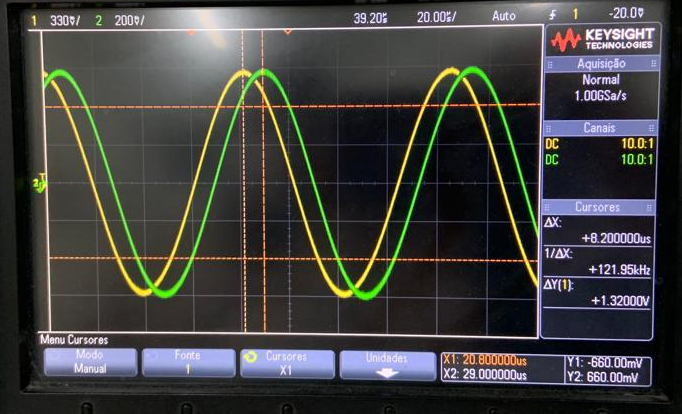
\includegraphics{circuito1.png}
\end{adjustbox}

\subparagraph*{Como podemos ver, há uma diferença de fase entre a tensão e a corrente, que era o resultado esperado.}

\subparagraph*{Observamos esta diferença de fase como $35.4$ graus. Ou $0.618rad$}



\subsection*{Segundo circuito}
\subparagraph*{Foto do gráfico da tensão e corrente observados abaixo.}
\subparagraph*{}
\begin{adjustbox}{scale=0.3}
    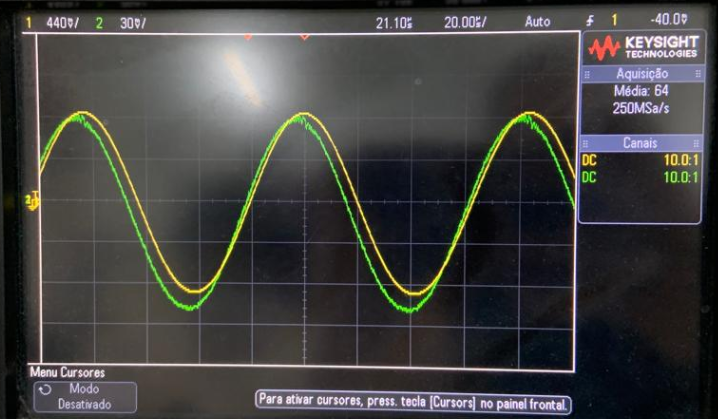
\includegraphics{circuito2.png}
\end{adjustbox}

\subparagraph*{Já neste o esperado era que estivessem em fase, salvo erros de medição e erros nos valores dos componentes utilizados.}

\subparagraph*{Observamos esta diferença de fase como $11.2$ graus. Ou $0.196$ rad.}

\end{document}